\documentclass[11pt,fleqn]{article} 
\usepackage[margin=0.8in, head=0.8in]{geometry} 
\usepackage{amsmath, amssymb, amsthm}
\usepackage{fancyhdr} 
\usepackage{palatino, url, multicol}
\usepackage{graphicx, pgfplots} 
\usepackage[all]{xy}
\usepackage{polynom} 
\usepackage[parfill]{parskip}
%\usepackage{pdfsync} %% I don't know why this messes up tabular column widths
\usepackage{enumerate}
\usepackage{framed}
\usepackage{setspace}
\usepackage{array}
\usepackage{pgf,tikz}
\usepackage{mathrsfs}
\usetikzlibrary{arrows}

\usetikzlibrary{calc}

\pgfplotsset{compat=1.6}

\pgfplotsset{soldot/.style={color=blue,only marks,mark=*}} \pgfplotsset{holdot/.style={color=blue,fill=white,only marks,mark=*}}

\renewcommand{\headrulewidth}{0pt}
\newcommand{\blank}[1]{\rule{#1}{0.75pt}}
\newcommand{\bc}{\begin{center}}
\newcommand{\ec}{\end{center}}
\newcommand{\be}{\begin{enumerate}}
\newcommand{\ee}{\end{enumerate}}

\newcommand{\ds}{\displaystyle}



\pagestyle{fancy} 
%\lfoot{Uses a calculator}
\rfoot{4-3 Sketch using derivatives}

\begin{document}
\begin{center}
  \LARGE
  \sc{4-3 Sketching Functions using Derivatives}\\
\end{center}

\begin{footnotesize}
\renewcommand\arraystretch{1.5}
\begin{tabular}{|p{.55\linewidth} | p{.4\linewidth}|} \hline
{\bf property of $f$} & {\bf how to recognize it} \\
\hline
\hline
$f$ is \emph{increasing} on $(a,b)$ if $f(x_{1}) \geq f(x_{2})$ for all $x_{1}, x_{2}$ in $(a,b)$ & $f'(x) \geq 0$\\ \hline
$f$ is \emph{decreasing} on $(a,b)$ if $f(x_{1}) \leq f(x_{2})$ for all $x_{1}, x_{2}$ in $(a,b)$ & $f'(x) \leq 0$\\ \hline
$f$ is \emph{concave up} on $(a,b)$ if $f'(x)$ is increasing on $(a,b)$  & $f''(x) \geq 0$\\ \hline
$f$ is \emph{concave down} on $(a,b)$ if $f'(x)$ is decreasing on $(a,b)$ & $f''(x) \leq 0$\\ \hline
$f$ has a \emph{local maximum} at $x = c$ if $f(c) \geq f(x)$ for all $x$ near $c$ & $f'(c) = 0$ and $f'$ changes from $+$ to $-$ at $c$ $\iff f''(c) <0$ \\ \hline
$f$ has a \emph{local minimum} at $x = c$ if $f(c) \leq f(x)$ for all $x$ near $c$ & $f'(c) = 0$ and $f'$ changes from $-$ to $+$ at $c$ $\iff f''(c) > 0$ \\ \hline
$f$ has an \emph{inflection point} at $x = c$ if $f$ changes concavity at $c$ & $f'(c)$ has a local max or min $\iff f''(c) = 0$ and $f''$ changes sign at $c$ \\ \hline
\end{tabular}
\end{footnotesize}


Below are the graphs of the FIRST DERIVATIVE, $f'(x)$, and the SECOND DERIVATIVE, $f''(x)$, of some unknown function $f$. Note that $f'(x)$ is the solid curve and $f''(x)$ is the dashed curve.  (Assume the domain of all the functions is $(-\infty, \infty)$ and that the functions continue in the way that they are going outside the area shown.) Sketch the graph of $f(x)$ on the given axes, and identify all the information about $f(x)$ required in the table.

\begin{minipage}{.6\linewidth}
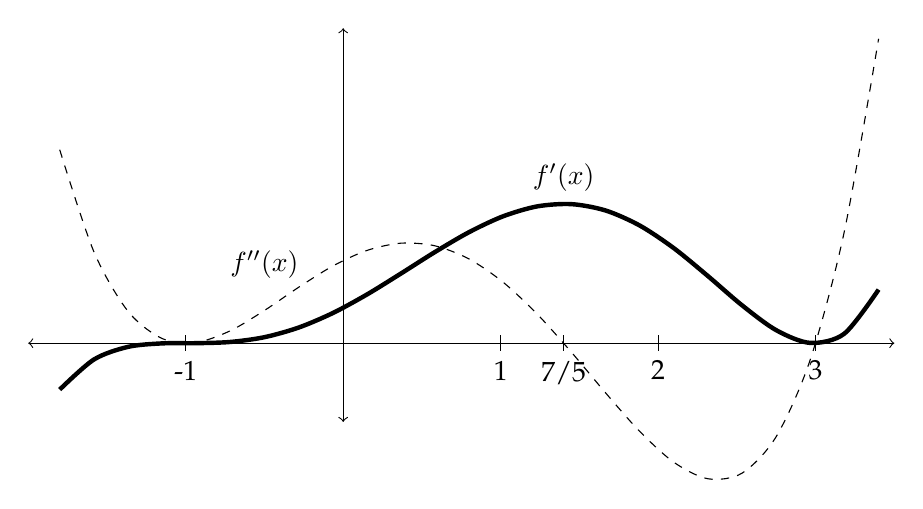
\begin{tikzpicture}[xscale=2]
\draw[<->](-2,0) -- (3.5,0);
\draw[<->](0,-1) -- (0,4);
\foreach \i in {-1,1,7/5,2,3}{\draw (\i,.1) -- (\i, -.1) node[below]{\i};}

\draw[ smooth, ultra thick, domain={-1.8:3.4}] plot (\x, {1/20*(\x+1)*(\x+1)*(\x+1)*(\x-3)*(\x-3)});
\draw (7/5, 2.1) node {$f'(x)$};

\draw[ smooth, dashed, domain={-1.8:3.4}] plot (\x, {1/20*(\x-3)*(1+\x)*(1+\x)*(5*\x-7)});

\draw (-1/2, 1) node {$f''(x)$};
\end{tikzpicture}

\bigskip

\begin{tikzpicture}[xscale=2]
\draw[<->](-2,0) -- (3.2,0);
\draw[<->](0,-1) -- (0,4);
\foreach \i in {-1,1,7/5,2,3}{\draw (\i,.1) -- (\i, -.1) node[below]{\i};}
\end{tikzpicture}
\end{minipage}
\hfill
\begin{minipage}{.3\linewidth}
\renewcommand\arraystretch{1.8}
\begin{tabular}{|p{.6\linewidth} | p{.4\linewidth}|}
\hline
{\bf property of $f$} & {\bf interval or point(s)}\\ \hline \hline
$f$ is increasing & \\ \hline
$f$ is decreasing & \\ \hline
$f$ has a local max & \\ \hline
$f$ has a local min & \\ \hline
$f$ is concave up & \\ \hline
$f$ is concave down& \\ \hline
$f$ has an inflection point & \\ \hline
\end{tabular}


\end{minipage}

\end{document}
